\documentclass[a4paper,12pt]{article}
\usepackage{amsmath}
\usepackage{amssymb}
\usepackage[polish]{babel}
\usepackage{polski}
\usepackage[utf8]{inputenc}
\usepackage{indentfirst}
\usepackage{geometry}
\usepackage{array}
\usepackage[pdftex]{color,graphicx}
\usepackage{subfigure}
\usepackage{afterpage}
\usepackage{setspace}
\usepackage{color}
\usepackage{wrapfig}
\usepackage{listings}
\usepackage{datetime}
\usepackage{color}

\renewcommand{\onehalfspacing}{\setstretch{1.6}}

\definecolor{Darkgreen}{rgb}{0.6,0.9,0.6}

\geometry{tmargin=2.5cm,bmargin=2.5cm,lmargin=2.5cm,rmargin=2.5cm}
\setlength{\parindent}{1cm}
\setlength{\parskip}{0mm}

\newenvironment{lista}{
\begin{itemize}
  \setlength{\itemsep}{1pt}
  \setlength{\parskip}{0pt}
  \setlength{\parsep}{0pt}
}{\end{itemize}}

\newcommand{\linia}{\rule{\linewidth}{0.4mm}}

\definecolor{lbcolor}{rgb}{0.95,0.95,0.95}
\lstset{
    backgroundcolor=\color{lbcolor},
    tabsize=4,
  language=C++,
  captionpos=b,
  tabsize=3,
  frame=lines,
  numbers=left,
  numberstyle=\tiny,
  numbersep=5pt,
  breaklines=true,
  showstringspaces=false,
  basicstyle=\footnotesize,
  identifierstyle=\color{magenta},
  keywordstyle=\color[rgb]{0,0,1},
  commentstyle=\color{Darkgreen},
  stringstyle=\color{red}
  }

\begin{document}

\noindent
\begin{tabular}{|c|p{11cm}|c|} \hline 
Grupa 6 & Wojciech Król, Maciej Kieruczenko & \ddmmyyyydate\today \tabularnewline
\hline 
\end{tabular}


\section*{Zadanie 3 - Liczby pierwsze - GPU}

Ćwiczenie polegało na przetestowaniu podanej bazy dużych liczb w celu sprawdzenia, które z nich należą do zbioru liczb pierwszych, a które do zbioru liczb złożonych. Program wykonano w technologii CUDA wykorzystując algorytm Millera-Rabina (Początkowo zaimplementowano sito Eratostenesa jednak ze względu na nie akceptowalny czas wymagany do wygenerowania wszystkich liczb pierwszych (liczby były przechowywane w tablicy całkowitej sprawdzanie a dostęp do poszczególnych odbywał się z użyciem maski bitowej) z danego przedziału zdecydowano się na opisany poniżej algorytm) .

Według definicji algorytm/test Millera-Rabina pozwala na sprawdzenie, czy interesująca nas liczba jest złożona, czy \textit{prawodpodobnie} pierwsza. Słowo "prawdopodobnie" jest tutaj bardzo ważne, ponieważ nigdy nie będziemy mieli 100-procentowej pewności, że test dokonał poprawnej oceny, jednakże mamy możliwość zwiększenia dokładności algorytmu poprzez zwiększenie liczby iteracji. 

Poniżej znajdują się kody najważniejszych funkcji wykonywanych na urządzeniu:
\begin{lstlisting}
__global__ void checkPrimeMillerRabin( curandState* globalState, unsigned int n,
    unsigned int d, int k, int s,unsigned int* result)
{
     int idx = threadIdx.x + blockIdx.x * blockDim.x;
     //If indx < k (precision) then Chceck number     
     while(idx<k)
     {
        checkPrimeNumber(globalState,n,d,s,result);
        if(*result != 0)
        {
            return;
        }
        idx+=blockDim.x * gridDim.x;  
    }
}

/**
Checks given number if prime (single iteration of Miller-Rabin algorithm)
**/
__device__ void checkPrimeNumber(curandState* globalState, unsigned int n,
    unsigned int d,int s,unsigned int* result)
{
    unsigned int a;
    //Get random int between 2 and n - 2
    rand(globalState,2, n-2,&a);
    unsigned int x;
    powerModulo(a,d,n,&x);
    if ( x == 1 || x == n-1 )
    {
        return;
    }
    for ( int i = 1; i <= s-1; ++i ) 
    {
        powerModulo(x, 2, n, &x);
        if ( x == 1 ) 
        {
            //Not a prime - return and set flag
            atomicAdd(result,1);
            return;
        }
        if ( x == n - 1 )
        {
            return;
        }
        //Check for other threads result.
        //Check every 10th iteration to avoid slow global memory acces
        if(i % 10 == 0 && *result != 0)
        {
            return;
        }
    }
    //Not a prime - set flag
    atomicAdd(result,1);
}
\end{lstlisting}

W tej części kodu wywoływana jest funkcja, w której dokonywane są obliczenia potrzebne do określenia, czy nasza liczba jest pierwsza. Powyższe metody wykonywane są ilość razy określoną w konstruktorze obiektu MillerRabinPrimeChecker:

\begin{lstlisting}
PrimeChecker *checker = new MillerRabinPrimeChecker(1000);
\end{lstlisting}

Ich wywołanie odbywa się w następujący sposób:

\begin{lstlisting}
setupRandom<<<10,35>>>(devStates,123,numberOfIterations);
checkPrimeMillerRabin<<<10,35>>>(devStates,n,d,numberOfIterations,s,devResult);
\end{lstlisting}

Testy były wykonywane na pliku udostępnionym przez prowadzącego na serwerze CUDA (1.txt). Liczbę bloków ustalono na 10, zaś dokładność obliczeń, a jednocześnie liczbę iteracji algorytmu ustawiono na 1000. Wyniki zestawiono w postaci dwóch wykresów - zależności czasu obliczeń oraz przyspieszenia od liczby wątków. Dodatkowo należy wspomnieć, że ze względu na brak wykorzystania pamięci współdzielonej i synchronizacji sposób podziału na gridy/bloki jest nie istotny - ważna jest jedynie sumaryczna liczba wątków.

\begin{figure}[!h]
	\centering
  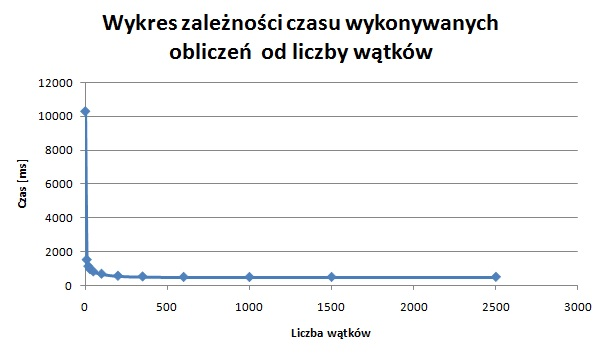
\includegraphics[width=0.6\textwidth]{1.jpg}
\end{figure}

\begin{figure}[!h]
	\centering
  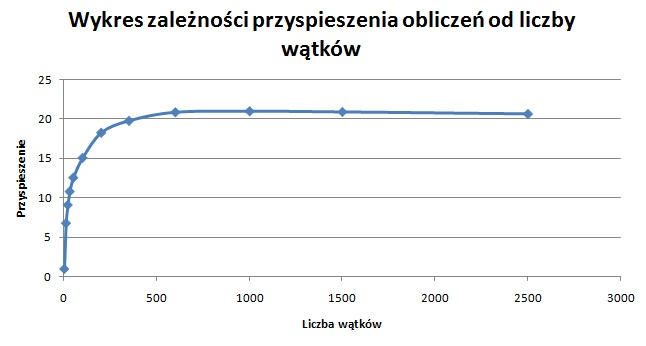
\includegraphics[width=0.6\textwidth]{2.jpg}
\end{figure}

Na podstawie powyższych wykresów można stwierdzić, że wyniki pomiaru czasu obliczeń są zgodne z oczekiwanymi. Dla niewielkiej ilości wątków wzrost przyspieszenia był bardzo gwałtowny, zaś poczynając od ok. 150-200 wątków zaczął się stabilizować na stałym poziomie. Powyżej 1000 wątków można było zaobserwować minimalne spadki wydajności, spowodowane uruchamianiem wątków, które nie wykonywały żadnych obliczeń.

Wnioski z wykonywanego ćwiczenia:
\begin{lista}
\item Dzięki zastosowaniu technologii CUDA można znacząco przyspieszyć czas obliczeń potrzebnych do określenia, czy podana duża liczba jest pierwsza (dla niewielkich pojedynczy wątek CPU będzie szybszy),
\item Większość testów sprawdzających czy liczba jest pierwsza, zapewniających zadowalającą wydajność, należy do grupy tzw. testów probabilistycznych, które nie są w stanie zagwarantować, że dokonana ocena jest poprawna, 
\item Najlepsze wyniki zaczęto osiągać dla łącznej ilości wątków zbliżonej lub większej (do pewnego momentu) liczbie jednostek obliczeniowych karty graficznej.
\end{lista}

\end{document}
